\documentclass[border=6pt]{standalone}
\usepackage{fontspec,xeCJK,amsmath,amssymb,tikz,graphicx}
\usetikzlibrary{arrows.meta}\setmainfont{Arial}\setCJKmainfont{PingFang SC}
\definecolor{ink}{HTML}{203340}\definecolor{blue}{HTML}{147E91}\definecolor{pale}{HTML}{EFF6F5}\definecolor{line}{HTML}{D3E0DF}
\begin{document}\begin{tikzpicture}[x=1cm,y=1cm,every node/.style={text=ink,font=\fontsize{10}{13}\selectfont}]
\path[use as bounding box](0,0)rectangle(11,29.2);\fill[pale](0,0)rectangle(11,29.2);
\node[font=\fontsize{19}{23}\selectfont\bfseries]at(5.5,28.4){ACT：一段动作，持续重算};
\node[text=blue]at(5.5,27.7){区域代码对应正文；虚线仅标阅读顺序};
\draw[rounded corners=6pt,draw=line,fill=white](.35,22.2)rectangle(10.65,27.0);\node[anchor=west,font=\fontsize{13}{16}\selectfont\bfseries]at(.65,26.45){A　示范与观察};
\node at(2.1,24.3){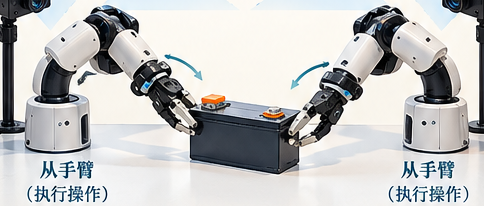
\includegraphics[width=2.75cm,height=2.7cm,keepaspectratio]{visual-1.png}};
\node[anchor=west]at(3.6,25.5){主臂关节目标 $\to$ 示范动作 $A_t:k\times14$};
\node[anchor=west]at(3.6,24.78){从臂关节 $q_t:14$；四路RGB $480\times640\times3$};
\node[anchor=west]at(3.6,24.06){50Hz目标；底层位置控制 $>1$kHz};
\node[anchor=west]at(3.6,23.34){对应正文 §3；相机观测另为30fps};
\draw[-{Stealth},dotted,draw=blue](5.5,22.2)--(5.5,21.8);
\draw[rounded corners=6pt,draw=line,fill=white](.35,17.0)rectangle(10.65,21.8);\node[anchor=west,font=\fontsize{13}{16}\selectfont\bfseries]at(.65,21.25){B　训练潜变量};
\node at(2.1,19.1){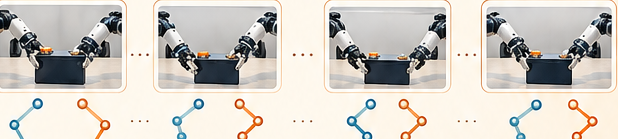
\includegraphics[width=2.75cm,height=2.7cm,keepaspectratio]{visual-2.png}};
\node[anchor=west]at(3.6,20.3){[CLS] + 关节 + 示范 $\to$ $(k+2)\times512$};
\node[anchor=west]at(3.6,19.580000000000002){4层Transformer $\to\mu,s\in\mathbb R^{32}$};
\node[anchor=west]at(3.6,18.86){重参数采样 $z=\mu+s\odot\epsilon$};
\node[anchor=west]at(3.6,18.14){仅训练使用；运行固定 $z=0$；正文 §4.3};
\draw[-{Stealth},dotted,draw=blue](5.5,17.0)--(5.5,16.6);
\draw[rounded corners=6pt,draw=line,fill=white](.35,11.8)rectangle(10.65,16.6);\node[anchor=west,font=\fontsize{13}{16}\selectfont\bfseries]at(.65,16.05){C　视觉到动作块};
\node at(2.1,13.900000000000002){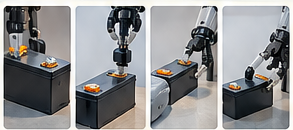
\includegraphics[width=2.75cm,height=2.7cm,keepaspectratio]{visual-3.png}};
\node[anchor=west]at(3.6,15.100000000000001){四图 $\to$ ResNet18 $\to$ $1200\times512$};
\node[anchor=west]at(3.6,14.38){加关节与z两个token $\to1202\times512$};
\node[anchor=west]at(3.6,13.660000000000002){4层编码 + 7层动作解码 $\to k\times14$};
\node[anchor=west]at(3.6,12.940000000000001){L1重建 + 10 KL；$k=100$；正文 §4.4};
\draw[-{Stealth},dotted,draw=blue](5.5,11.8)--(5.5,11.4);
\draw[rounded corners=6pt,draw=line,fill=white](.35,6.599999999999999)rectangle(10.65,11.399999999999999);\node[anchor=west,font=\fontsize{13}{16}\selectfont\bfseries]at(.65,10.849999999999998){D　同一时刻集成};
\node at(2.1,8.7){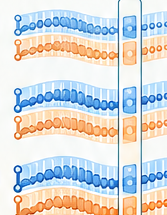
\includegraphics[width=2.75cm,height=2.7cm,keepaspectratio]{visual-4.png}};
\node[anchor=west]at(3.6,9.899999999999999){每步观察 $\to$ 新预测块；收同一时刻各预测};
\node[anchor=west]at(3.6,9.179999999999998){旧到新 $w_i=e^{-mi}$；归一化加权};
\node[anchor=west]at(3.6,8.459999999999999){一条14维目标 $\to$ 电机 $\to$ 新观察回C};
\node[anchor=west]at(3.6,7.739999999999998){100步预测，逐步闭环；正文 §4.1--4.2};
\draw[-{Stealth},dotted,draw=blue](5.5,6.599999999999999)--(5.5,6.199999999999998);
\draw[rounded corners=6pt,draw=line,fill=white](.35,1.3999999999999995)rectangle(10.65,6.199999999999999);\node[anchor=west,font=\fontsize{13}{16}\selectfont\bfseries]at(.65,5.6499999999999995){E　任务与消融};
\node at(2.1,3.499999999999999){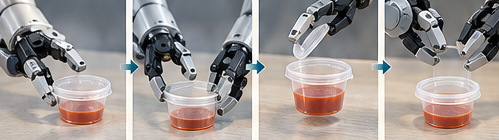
\includegraphics[width=2.75cm,height=2.7cm,keepaspectratio]{visual-5.png}};
\node[anchor=west]at(3.6,4.699999999999999){每任务训练；6项实机 + 2项仿真};
\node[anchor=west]at(3.6,3.9799999999999995){分清人遥操作、策略自主和消融设置};
\node[anchor=west]at(3.6,3.2599999999999993){对照分块、时间集成、CVAE与频率};
\node[anchor=west]at(3.6,2.539999999999999){读成功阶段和感知失败；正文 §5--7};
\end{tikzpicture}\end{document}